\documentclass[a4paper]{book}
\usepackage{makeidx}
\usepackage{natbib}
\usepackage{graphicx}
\usepackage{multicol}
\usepackage{float}
\usepackage{listings}
\usepackage{color}
\usepackage{ifthen}
\usepackage[table]{xcolor}
\usepackage{textcomp}
\usepackage{alltt}
\usepackage{ifpdf}
\ifpdf
\usepackage[pdftex,
            pagebackref=true,
            colorlinks=true,
            linkcolor=blue,
            unicode
           ]{hyperref}
\else
\usepackage[ps2pdf,
            pagebackref=true,
            colorlinks=true,
            linkcolor=blue,
            unicode
           ]{hyperref}
\usepackage{pspicture}
\fi
\usepackage[utf8]{inputenc}
\usepackage{mathptmx}
\usepackage[scaled=.90]{helvet}
\usepackage{courier}
\usepackage{sectsty}
\usepackage[titles]{tocloft}
\usepackage{doxygen}
\lstset{language=C++,inputencoding=utf8,basicstyle=\footnotesize,breaklines=true,breakatwhitespace=true,tabsize=8,numbers=left }
\makeindex
\setcounter{tocdepth}{3}
\renewcommand{\footrulewidth}{0.4pt}
\renewcommand{\familydefault}{\sfdefault}
\hfuzz=15pt
\setlength{\emergencystretch}{15pt}
\hbadness=750
\tolerance=750
\begin{document}
\hypersetup{pageanchor=false,citecolor=blue}
\begin{titlepage}
\vspace*{7cm}
\begin{center}
{\Large spiri api \\[1ex]\large 1.\-1.\-2 }\\
\vspace*{1cm}
{\large \-Generated by Doxygen 1.7.6.1}\\
\vspace*{0.5cm}
{\small Wed Aug 6 2014 14:33:13}\\
\end{center}
\end{titlepage}
\clearemptydoublepage
\pagenumbering{roman}
\tableofcontents
\clearemptydoublepage
\pagenumbering{arabic}
\hypersetup{pageanchor=true,citecolor=blue}
\chapter{\-Todo \-List}
\label{todo}
\hypertarget{todo}{}

\begin{DoxyRefList}
\item[\label{todo__todo000001}%
\hypertarget{todo__todo000001}{}%
Member \hyperlink{classspiri__api_1_1get__state_1_1_staterobot_a015efa1f3a59211063e167ec0cb1fc3b}{spiri\-\_\-api.get\-\_\-state.Staterobot.\-\_\-\-\_\-init\-\_\-\-\_\-} ]The callback needs to be called before the user can send goals. 
\item[\label{todo__todo000002}%
\hypertarget{todo__todo000002}{}%
Member \hyperlink{classspiri__api_1_1get__state_1_1_staterobot_af6d1fe436714134bbd2fb78da0b09835}{spiri\-\_\-api.get\-\_\-state.Staterobot.send\-\_\-goal} ]Return based something on success or failure 

This function should also take in G\-P\-S coordinates 
\begin{DoxyParams}{Parameters}
{\em x} & coordinate in x axis \\
\hline
{\em y} & coordinate in y axis \\
\hline
{\em z} & coordinate in z axis  \\
\hline
\end{DoxyParams}

\item[\label{todo__todo000003}%
\hypertarget{todo__todo000003}{}%
Member \hyperlink{classspiri__api_1_1get__state_1_1_staterobot_abc35e5157bb27bfc35bbfb4aee9df2e5}{spiri\-\_\-api.get\-\_\-state.Staterobot.send\-\_\-goal\-\_\-relative\-\_\-threading} ]Return based something on success or failure 
\begin{DoxyParams}{Parameters}
{\em x} & distance in metres in x axis \\
\hline
{\em y} & distance in metres in y axis \\
\hline
{\em z} & distance in metres in z axis  \\
\hline
\end{DoxyParams}

\item[\label{todo__todo000004}%
\hypertarget{todo__todo000004}{}%
Member \hyperlink{class_staterobot_addfc245d53239eed664812a50a916428}{Staterobot\-:\-:send\-\_\-vel} (float x, float y, float z)]This is hack. If there exists a better way in R\-O\-S need to find that 
\end{DoxyRefList}
\chapter{\-Namespace \-Index}
\section{Namespace List}
Here is a list of all documented namespaces with brief descriptions\-:\begin{DoxyCompactList}
\item\contentsline{section}{\hyperlink{namespacespiri__api}{spiri\-\_\-api} \\*A\-P\-I for Spiri }{\pageref{namespacespiri__api}}{}
\end{DoxyCompactList}

\chapter{\-Class \-Index}
\section{\-Class \-List}
\-Here are the classes, structs, unions and interfaces with brief descriptions\-:\begin{DoxyCompactList}
\item\contentsline{section}{\hyperlink{classspiri__api_1_1camera_1_1camera__interface}{spiri\-\_\-api.\-camera.\-camera\-\_\-interface} \\*\-Class defining all the functions for perception }{\pageref{classspiri__api_1_1camera_1_1camera__interface}}{}
\item\contentsline{section}{\hyperlink{classspiri__api_1_1pid_1_1_p_i_d}{spiri\-\_\-api.\-pid.\-P\-I\-D} }{\pageref{classspiri__api_1_1pid_1_1_p_i_d}}{}
\item\contentsline{section}{\hyperlink{class_staterobot}{\-Staterobot} }{\pageref{class_staterobot}}{}
\item\contentsline{section}{\hyperlink{classspiri__api_1_1get__state_1_1_staterobot}{spiri\-\_\-api.\-get\-\_\-state.\-Staterobot} \\*\-Class defining all the functions to control \-Spiri }{\pageref{classspiri__api_1_1get__state_1_1_staterobot}}{}
\item\contentsline{section}{\hyperlink{classspiri__api_1_1figure__movement_1_1_staterobot}{spiri\-\_\-api.\-figure\-\_\-movement.\-Staterobot} }{\pageref{classspiri__api_1_1figure__movement_1_1_staterobot}}{}
\item\contentsline{section}{\hyperlink{classspiri__api_1_1request_1_1_staterobot}{spiri\-\_\-api.\-request.\-Staterobot} }{\pageref{classspiri__api_1_1request_1_1_staterobot}}{}
\end{DoxyCompactList}

\chapter{\-Namespace \-Documentation}
\hypertarget{namespacespiri__api}{\section{spiri\-\_\-api Namespace Reference}
\label{namespacespiri__api}\index{spiri\-\_\-api@{spiri\-\_\-api}}
}


A\-P\-I for Spiri.  




\subsection{Detailed Description}
A\-P\-I for Spiri. \begin{DoxyAuthor}{Author}
Rohan Bhargava 
\end{DoxyAuthor}
\begin{DoxyVersion}{Version}
1.\-1.\-1 
\end{DoxyVersion}

\chapter{\-Class \-Documentation}
\hypertarget{classspiri__api_1_1camera_1_1camera__interface}{\section{spiri\-\_\-api.\-camera.\-camera\-\_\-interface \-Class \-Reference}
\label{classspiri__api_1_1camera_1_1camera__interface}\index{spiri\-\_\-api.\-camera.\-camera\-\_\-interface@{spiri\-\_\-api.\-camera.\-camera\-\_\-interface}}
}


\-Class defining all the functions for perception.  


\subsection*{\-Public \-Member \-Functions}
\begin{DoxyCompactItemize}
\item 
\hypertarget{classspiri__api_1_1camera_1_1camera__interface_af1f1cc7fbff0ec085b45dfb0922c691f}{def \hyperlink{classspiri__api_1_1camera_1_1camera__interface_af1f1cc7fbff0ec085b45dfb0922c691f}{\-\_\-\-\_\-init\-\_\-\-\_\-}}\label{classspiri__api_1_1camera_1_1camera__interface_af1f1cc7fbff0ec085b45dfb0922c691f}

\begin{DoxyCompactList}\small\item\em \-Constructor. \end{DoxyCompactList}\item 
def \hyperlink{classspiri__api_1_1camera_1_1camera__interface_aa01883759da88698cfa72cb7988167c7}{callback\-\_\-threading}
\begin{DoxyCompactList}\small\item\em start the threads \end{DoxyCompactList}\item 
\hypertarget{classspiri__api_1_1camera_1_1camera__interface_a35fb0ce651203d6fe53c3db90684ee92}{def {\bfseries callback\-\_\-left}}\label{classspiri__api_1_1camera_1_1camera__interface_a35fb0ce651203d6fe53c3db90684ee92}

\item 
\hypertarget{classspiri__api_1_1camera_1_1camera__interface_aed778f8b52482e9c0f2882335cbdf81d}{def {\bfseries callback\-\_\-right}}\label{classspiri__api_1_1camera_1_1camera__interface_aed778f8b52482e9c0f2882335cbdf81d}

\item 
\hypertarget{classspiri__api_1_1camera_1_1camera__interface_abc6c919fb016eddbb6885f5ca0b7e52b}{def {\bfseries callback\-\_\-bottom}}\label{classspiri__api_1_1camera_1_1camera__interface_abc6c919fb016eddbb6885f5ca0b7e52b}

\item 
\hypertarget{classspiri__api_1_1camera_1_1camera__interface_a53d57fe7e17a2eb52649ac2319c01f34}{def {\bfseries get\-\_\-left\-\_\-image}}\label{classspiri__api_1_1camera_1_1camera__interface_a53d57fe7e17a2eb52649ac2319c01f34}

\item 
\hypertarget{classspiri__api_1_1camera_1_1camera__interface_a72194dfd1f91a4b7ddaf93581a21c51d}{def {\bfseries get\-\_\-right\-\_\-image}}\label{classspiri__api_1_1camera_1_1camera__interface_a72194dfd1f91a4b7ddaf93581a21c51d}

\item 
\hypertarget{classspiri__api_1_1camera_1_1camera__interface_a1b4e9974e651b63dca9b7b28a5f80dc8}{def {\bfseries get\-\_\-bottom\-\_\-image}}\label{classspiri__api_1_1camera_1_1camera__interface_a1b4e9974e651b63dca9b7b28a5f80dc8}

\item 
\hypertarget{classspiri__api_1_1camera_1_1camera__interface_ab33d6fc726b927d453beee3e0db42d07}{def {\bfseries save\-\_\-left\-\_\-image\-\_\-threading}}\label{classspiri__api_1_1camera_1_1camera__interface_ab33d6fc726b927d453beee3e0db42d07}

\item 
\hypertarget{classspiri__api_1_1camera_1_1camera__interface_adc7924738ace2d72573ba20cab60bee1}{def {\bfseries save\-\_\-left\-\_\-image}}\label{classspiri__api_1_1camera_1_1camera__interface_adc7924738ace2d72573ba20cab60bee1}

\item 
\hypertarget{classspiri__api_1_1camera_1_1camera__interface_aed21830ab1c54288131fc6880496a43c}{def {\bfseries save\-\_\-right\-\_\-image}}\label{classspiri__api_1_1camera_1_1camera__interface_aed21830ab1c54288131fc6880496a43c}

\item 
\hypertarget{classspiri__api_1_1camera_1_1camera__interface_a150da32f002ae666ac00c5a81a43234d}{def {\bfseries save\-\_\-bottom\-\_\-image}}\label{classspiri__api_1_1camera_1_1camera__interface_a150da32f002ae666ac00c5a81a43234d}

\item 
def \hyperlink{classspiri__api_1_1camera_1_1camera__interface_aa218b82e6e2135a1c0e7011edc9889cf}{save\-\_\-left\-\_\-video}
\begin{DoxyCompactList}\small\item\em \-Functions to record video for a given time. \end{DoxyCompactList}\end{DoxyCompactItemize}
\subsection*{\-Public \-Attributes}
\begin{DoxyCompactItemize}
\item 
\hypertarget{classspiri__api_1_1camera_1_1camera__interface_a5bd8c6fc7e7fff36c408f3d4effb0cd4}{{\bfseries left\-\_\-image}}\label{classspiri__api_1_1camera_1_1camera__interface_a5bd8c6fc7e7fff36c408f3d4effb0cd4}

\item 
\hypertarget{classspiri__api_1_1camera_1_1camera__interface_a884adfeef30750273d4bf3cb376e554d}{{\bfseries right\-\_\-image}}\label{classspiri__api_1_1camera_1_1camera__interface_a884adfeef30750273d4bf3cb376e554d}

\item 
\hypertarget{classspiri__api_1_1camera_1_1camera__interface_af588921d264de69b2f5400a91aabd307}{{\bfseries bottom\-\_\-image}}\label{classspiri__api_1_1camera_1_1camera__interface_af588921d264de69b2f5400a91aabd307}

\item 
\hypertarget{classspiri__api_1_1camera_1_1camera__interface_acc72b69b3e57e819a8c29e5b8d9dd604}{{\bfseries bridge}}\label{classspiri__api_1_1camera_1_1camera__interface_acc72b69b3e57e819a8c29e5b8d9dd604}

\item 
\hypertarget{classspiri__api_1_1camera_1_1camera__interface_a07bd4664b67aee3ccf48ccf40cb0eea4}{{\bfseries number}}\label{classspiri__api_1_1camera_1_1camera__interface_a07bd4664b67aee3ccf48ccf40cb0eea4}

\item 
\hypertarget{classspiri__api_1_1camera_1_1camera__interface_a13b6113c5c2072d08ddb5901a4d02449}{{\bfseries cv\-\_\-image\-\_\-left}}\label{classspiri__api_1_1camera_1_1camera__interface_a13b6113c5c2072d08ddb5901a4d02449}

\item 
\hypertarget{classspiri__api_1_1camera_1_1camera__interface_ade9f1dde3c488e2e47074034ddb965e1}{{\bfseries cv\-\_\-image\-\_\-right}}\label{classspiri__api_1_1camera_1_1camera__interface_ade9f1dde3c488e2e47074034ddb965e1}

\item 
\hypertarget{classspiri__api_1_1camera_1_1camera__interface_a723d3924c26e8d21ed6c13916c3db41c}{{\bfseries cv\-\_\-image\-\_\-bottom}}\label{classspiri__api_1_1camera_1_1camera__interface_a723d3924c26e8d21ed6c13916c3db41c}

\end{DoxyCompactItemize}


\subsection{\-Detailed \-Description}
\-Class defining all the functions for perception. 

\subsection{\-Member \-Function \-Documentation}
\hypertarget{classspiri__api_1_1camera_1_1camera__interface_aa01883759da88698cfa72cb7988167c7}{\index{spiri\-\_\-api\-::camera\-::camera\-\_\-interface@{spiri\-\_\-api\-::camera\-::camera\-\_\-interface}!callback\-\_\-threading@{callback\-\_\-threading}}
\index{callback\-\_\-threading@{callback\-\_\-threading}!spiri_api::camera::camera_interface@{spiri\-\_\-api\-::camera\-::camera\-\_\-interface}}
\subsubsection[{callback\-\_\-threading}]{\setlength{\rightskip}{0pt plus 5cm}def {\bf spiri\-\_\-api.\-camera.\-camera\-\_\-interface.\-callback\-\_\-threading} (
\begin{DoxyParamCaption}
\item[{}]{self}
\end{DoxyParamCaption}
)}}\label{classspiri__api_1_1camera_1_1camera__interface_aa01883759da88698cfa72cb7988167c7}


start the threads 

\begin{DoxyRefDesc}{\-Todo}
\item[\hyperlink{todo__todo000001}{\-Todo}]\-Can create threads for every subscriber \end{DoxyRefDesc}
\hypertarget{classspiri__api_1_1camera_1_1camera__interface_aa218b82e6e2135a1c0e7011edc9889cf}{\index{spiri\-\_\-api\-::camera\-::camera\-\_\-interface@{spiri\-\_\-api\-::camera\-::camera\-\_\-interface}!save\-\_\-left\-\_\-video@{save\-\_\-left\-\_\-video}}
\index{save\-\_\-left\-\_\-video@{save\-\_\-left\-\_\-video}!spiri_api::camera::camera_interface@{spiri\-\_\-api\-::camera\-::camera\-\_\-interface}}
\subsubsection[{save\-\_\-left\-\_\-video}]{\setlength{\rightskip}{0pt plus 5cm}def {\bf spiri\-\_\-api.\-camera.\-camera\-\_\-interface.\-save\-\_\-left\-\_\-video} (
\begin{DoxyParamCaption}
\item[{}]{self, }
\item[{}]{path = {\ttfamily './left\-\_\-video.avi'}, }
\item[{}]{period = {\ttfamily '10'}}
\end{DoxyParamCaption}
)}}\label{classspiri__api_1_1camera_1_1camera__interface_aa218b82e6e2135a1c0e7011edc9889cf}


\-Functions to record video for a given time. 

\begin{DoxyRefDesc}{\-Todo}
\item[\hyperlink{todo__todo000002}{\-Todo}]the sleep function is a hack.\end{DoxyRefDesc}
\-Need to find a better way 

\-The documentation for this class was generated from the following file\-:\begin{DoxyCompactItemize}
\item 
src/spiri\-\_\-api/camera.\-py\end{DoxyCompactItemize}

\hypertarget{classspiri__api_1_1pid_1_1_p_i_d}{\section{spiri\-\_\-api.\-pid.\-P\-I\-D \-Class \-Reference}
\label{classspiri__api_1_1pid_1_1_p_i_d}\index{spiri\-\_\-api.\-pid.\-P\-I\-D@{spiri\-\_\-api.\-pid.\-P\-I\-D}}
}
\subsection*{\-Public \-Member \-Functions}
\begin{DoxyCompactItemize}
\item 
\hypertarget{classspiri__api_1_1pid_1_1_p_i_d_a1caafcce2de3920b8e3d7a3c819f30a7}{def {\bfseries \-\_\-\-\_\-init\-\_\-\-\_\-}}\label{classspiri__api_1_1pid_1_1_p_i_d_a1caafcce2de3920b8e3d7a3c819f30a7}

\item 
def \hyperlink{classspiri__api_1_1pid_1_1_p_i_d_a7e0273463b18d2f0ddef7f91c8457ea9}{update}
\item 
def \hyperlink{classspiri__api_1_1pid_1_1_p_i_d_ae1ae6a13b63865567c271c0eb2118fa2}{set\-Point}
\end{DoxyCompactItemize}
\subsection*{\-Public \-Attributes}
\begin{DoxyCompactItemize}
\item 
\hypertarget{classspiri__api_1_1pid_1_1_p_i_d_a864d9dad88cbae64cdef3acd7b5c48a7}{{\bfseries \-Kp}}\label{classspiri__api_1_1pid_1_1_p_i_d_a864d9dad88cbae64cdef3acd7b5c48a7}

\item 
\hypertarget{classspiri__api_1_1pid_1_1_p_i_d_a3a732769525c841bc71afc58eefcf494}{{\bfseries \-Ki}}\label{classspiri__api_1_1pid_1_1_p_i_d_a3a732769525c841bc71afc58eefcf494}

\item 
\hypertarget{classspiri__api_1_1pid_1_1_p_i_d_a3a55806697a84e00d5cf34678d8b0ff9}{{\bfseries \-Kd}}\label{classspiri__api_1_1pid_1_1_p_i_d_a3a55806697a84e00d5cf34678d8b0ff9}

\item 
\hypertarget{classspiri__api_1_1pid_1_1_p_i_d_a261c5efafdc8137f6ad2992136c449e0}{{\bfseries \-Derivator}}\label{classspiri__api_1_1pid_1_1_p_i_d_a261c5efafdc8137f6ad2992136c449e0}

\item 
\hypertarget{classspiri__api_1_1pid_1_1_p_i_d_a2cd923ae760a6ede8232e46348abc474}{{\bfseries \-Integrator}}\label{classspiri__api_1_1pid_1_1_p_i_d_a2cd923ae760a6ede8232e46348abc474}

\item 
\hypertarget{classspiri__api_1_1pid_1_1_p_i_d_a9a49de2c1cd0a7b22957236d4cff3635}{{\bfseries \-Integrator\-\_\-max}}\label{classspiri__api_1_1pid_1_1_p_i_d_a9a49de2c1cd0a7b22957236d4cff3635}

\item 
\hypertarget{classspiri__api_1_1pid_1_1_p_i_d_a4914219a7c5d3316fa5adca23b8d8588}{{\bfseries \-Integrator\-\_\-min}}\label{classspiri__api_1_1pid_1_1_p_i_d_a4914219a7c5d3316fa5adca23b8d8588}

\item 
\hypertarget{classspiri__api_1_1pid_1_1_p_i_d_a601670802f7c407cb7dfabc0610bd241}{{\bfseries set\-\_\-point}}\label{classspiri__api_1_1pid_1_1_p_i_d_a601670802f7c407cb7dfabc0610bd241}

\item 
\hypertarget{classspiri__api_1_1pid_1_1_p_i_d_aae228001def6dc887d812dc4ee48bb65}{{\bfseries error}}\label{classspiri__api_1_1pid_1_1_p_i_d_aae228001def6dc887d812dc4ee48bb65}

\item 
\hypertarget{classspiri__api_1_1pid_1_1_p_i_d_aceb675ce34e8c306b5356ae5e294affd}{{\bfseries \-P\-\_\-value}}\label{classspiri__api_1_1pid_1_1_p_i_d_aceb675ce34e8c306b5356ae5e294affd}

\item 
\hypertarget{classspiri__api_1_1pid_1_1_p_i_d_a62f3f6c2a9f902195d4600d6d9f7a9fa}{{\bfseries \-D\-\_\-value}}\label{classspiri__api_1_1pid_1_1_p_i_d_a62f3f6c2a9f902195d4600d6d9f7a9fa}

\end{DoxyCompactItemize}


\subsection{\-Detailed \-Description}
\begin{DoxyVerb}
Discrete PID control
\end{DoxyVerb}
 

\subsection{\-Member \-Function \-Documentation}
\hypertarget{classspiri__api_1_1pid_1_1_p_i_d_ae1ae6a13b63865567c271c0eb2118fa2}{\index{spiri\-\_\-api\-::pid\-::\-P\-I\-D@{spiri\-\_\-api\-::pid\-::\-P\-I\-D}!set\-Point@{set\-Point}}
\index{set\-Point@{set\-Point}!spiri_api::pid::PID@{spiri\-\_\-api\-::pid\-::\-P\-I\-D}}
\subsubsection[{set\-Point}]{\setlength{\rightskip}{0pt plus 5cm}def {\bf spiri\-\_\-api.\-pid.\-P\-I\-D.\-set\-Point} (
\begin{DoxyParamCaption}
\item[{}]{self, }
\item[{}]{set\-\_\-point}
\end{DoxyParamCaption}
)}}\label{classspiri__api_1_1pid_1_1_p_i_d_ae1ae6a13b63865567c271c0eb2118fa2}
\begin{DoxyVerb}
Initilize the setpoint of PID
\end{DoxyVerb}
 \hypertarget{classspiri__api_1_1pid_1_1_p_i_d_a7e0273463b18d2f0ddef7f91c8457ea9}{\index{spiri\-\_\-api\-::pid\-::\-P\-I\-D@{spiri\-\_\-api\-::pid\-::\-P\-I\-D}!update@{update}}
\index{update@{update}!spiri_api::pid::PID@{spiri\-\_\-api\-::pid\-::\-P\-I\-D}}
\subsubsection[{update}]{\setlength{\rightskip}{0pt plus 5cm}def {\bf spiri\-\_\-api.\-pid.\-P\-I\-D.\-update} (
\begin{DoxyParamCaption}
\item[{}]{self, }
\item[{}]{current\-\_\-value}
\end{DoxyParamCaption}
)}}\label{classspiri__api_1_1pid_1_1_p_i_d_a7e0273463b18d2f0ddef7f91c8457ea9}
\begin{DoxyVerb}
Calculate PID output value for given reference input and feedback
\end{DoxyVerb}
 

\-The documentation for this class was generated from the following file\-:\begin{DoxyCompactItemize}
\item 
src/spiri\-\_\-api/pid.\-py\end{DoxyCompactItemize}

\hypertarget{class_staterobot}{\section{Staterobot Class Reference}
\label{class_staterobot}\index{Staterobot@{Staterobot}}
}


Collaboration diagram for Staterobot\-:
\nopagebreak
\begin{figure}[H]
\begin{center}
\leavevmode
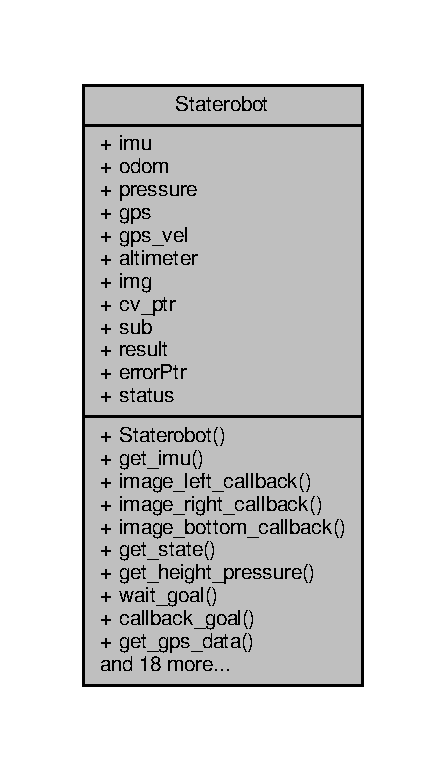
\includegraphics[width=214pt]{class_staterobot__coll__graph}
\end{center}
\end{figure}
\subsection*{Public Member Functions}
\begin{DoxyCompactItemize}
\item 
\hyperlink{class_staterobot_ab99a92f98d724c96989a744aee273155}{Staterobot} ()
\item 
std\-::vector$<$ double $>$ \hyperlink{class_staterobot_a50e002ec81917b295a87463127648a52}{get\-\_\-imu} ()
\item 
\hypertarget{class_staterobot_a4cb41f60186d02b210f354d0199584a4}{void {\bfseries image\-\_\-left\-\_\-callback} (const sensor\-\_\-msgs\-::\-Image\-Const\-Ptr \&)}\label{class_staterobot_a4cb41f60186d02b210f354d0199584a4}

\item 
\hypertarget{class_staterobot_af908b8a70811f3c0a48efe323610602d}{void {\bfseries image\-\_\-right\-\_\-callback} (const sensor\-\_\-msgs\-::\-Image\-Const\-Ptr \&)}\label{class_staterobot_af908b8a70811f3c0a48efe323610602d}

\item 
\hypertarget{class_staterobot_a8ad49fe9f855e5874d8736067fa7fac0}{void {\bfseries image\-\_\-bottom\-\_\-callback} (const sensor\-\_\-msgs\-::\-Image\-Const\-Ptr \&)}\label{class_staterobot_a8ad49fe9f855e5874d8736067fa7fac0}

\item 
std\-::vector$<$ double $>$ \hyperlink{class_staterobot_a51670cc44348eae6328f220421ea328f}{get\-\_\-state} ()
\item 
float \hyperlink{class_staterobot_a0318f7abf24c5c60aee915224af6af02}{get\-\_\-height\-\_\-pressure} ()
\item 
\hypertarget{class_staterobot_a4a44c24dd5cdb773aa40772d02b41720}{bool {\bfseries wait\-\_\-goal} ()}\label{class_staterobot_a4a44c24dd5cdb773aa40772d02b41720}

\item 
\hypertarget{class_staterobot_a37cbdfcb1cc30194f0fa0742952a0aad}{void {\bfseries callback\-\_\-goal} (const action\-\_\-controller\-::\-Multi\-Dof\-Follow\-Joint\-Trajectory\-Action\-Result\-Ptr \&)}\label{class_staterobot_a37cbdfcb1cc30194f0fa0742952a0aad}

\item 
std\-::vector$<$ double $>$ \hyperlink{class_staterobot_a31dcc23cfb620c95e58f3b5ad4bb6b6d}{get\-\_\-gps\-\_\-data} ()
\item 
std\-::vector$<$ double $>$ \hyperlink{class_staterobot_a3a9ee7a49cbb278ffc5f3b201dcae951}{get\-\_\-gps\-\_\-vel} ()
\item 
float \hyperlink{class_staterobot_a3e92b9d6f17c0812e8ed435602d1f717}{get\-\_\-height\-\_\-altimeter} ()
\item 
bool \hyperlink{class_staterobot_a4f1aff1c608a045faa07fa8b9cff4b65}{send\-\_\-goal} (float x, float y, float z, bool relative)
\item 
cv\-::\-Mat \hyperlink{class_staterobot_a5b0323154aa0a19ed82b02cfe7376974}{get\-\_\-left\-\_\-image} ()
\item 
cv\-::\-Mat \hyperlink{class_staterobot_ab1d8f9bfdbd766b96110c0a65fe08f43}{get\-\_\-right\-\_\-image} ()
\item 
cv\-::\-Mat \hyperlink{class_staterobot_a310b2c9315316f96054357ebb705438f}{get\-\_\-bottom\-\_\-image} ()
\item 
void \hyperlink{class_staterobot_a1da31a1c7a8f39878d2511ca86adeb8f}{save\-\_\-image} (const std\-::string, const std\-::string)
\item 
void \hyperlink{class_staterobot_addfc245d53239eed664812a50a916428}{send\-\_\-vel} (float x, float y, float z)
\item 
boost\-::python\-::list \hyperlink{class_staterobot_a3e6bd1883c62204de398342cf8004351}{get\-\_\-imu\-\_\-python} ()
\item 
boost\-::python\-::list \hyperlink{class_staterobot_a91206b2bef7c39193df2eef7b8bae523}{get\-\_\-state\-\_\-python} ()
\item 
boost\-::python\-::list \hyperlink{class_staterobot_ac2fe6ca526d21c1bcb2e284f000759a4}{get\-\_\-gps\-\_\-data\-\_\-python} ()
\item 
boost\-::python\-::list \hyperlink{class_staterobot_aed3a2e6aa076fe6e38f97eb9ab9ef41a}{get\-\_\-gps\-\_\-vel\-\_\-python} ()
\item 
std\-::string \hyperlink{class_staterobot_ab7e02e341f1f3ccfaaa322a2fc1e2caf}{get\-\_\-left\-\_\-image\-\_\-python} ()
\item 
std\-::string \hyperlink{class_staterobot_ab222942f5fe07919fc4999eb600706d1}{get\-\_\-right\-\_\-image\-\_\-python} ()
\item 
std\-::string \hyperlink{class_staterobot_a36d188439ca66b3e56cff58877297945}{get\-\_\-bottom\-\_\-image\-\_\-python} ()
\item 
bool \hyperlink{class_staterobot_abc938e713a748e1803a304e30145e3d1}{send\-\_\-goal\-\_\-python} (boost\-::python\-::list \&)
\item 
bool \hyperlink{class_staterobot_a5ec7a1fdfa9757ddea8c1587e8324f4a}{send\-\_\-goal\-\_\-python\-\_\-relative} (boost\-::python\-::list \&)
\item 
void \hyperlink{class_staterobot_ae47718241f57b27cf4854730cfb50201}{send\-\_\-vel\-\_\-python} (boost\-::python\-::list \&)
\end{DoxyCompactItemize}
\subsection*{Public Attributes}
\begin{DoxyCompactItemize}
\item 
\hypertarget{class_staterobot_ae6075d8fe1f2714e62f98ecfcfabab5f}{sensor\-\_\-msgs\-::\-Imu\-Const\-Ptr {\bfseries imu}}\label{class_staterobot_ae6075d8fe1f2714e62f98ecfcfabab5f}

\item 
\hypertarget{class_staterobot_a647d9af50a8896f64fa9456b5719157b}{nav\-\_\-msgs\-::\-Odometry\-Const\-Ptr {\bfseries odom}}\label{class_staterobot_a647d9af50a8896f64fa9456b5719157b}

\item 
\hypertarget{class_staterobot_a8ab2546d67712dbed7d288f66430d923}{geometry\-\_\-msgs\-::\-Point\-Stamped\-Const\-Ptr {\bfseries pressure}}\label{class_staterobot_a8ab2546d67712dbed7d288f66430d923}

\item 
\hypertarget{class_staterobot_aaade9f6f0d32fb6baaef1c745fa138de}{sensor\-\_\-msgs\-::\-Nav\-Sat\-Fix\-Const\-Ptr {\bfseries gps}}\label{class_staterobot_aaade9f6f0d32fb6baaef1c745fa138de}

\item 
\hypertarget{class_staterobot_a78d4a58c9335c40740c830f7d8499c75}{geometry\-\_\-msgs\-::\-Vector3\-Stamped\-Const\-Ptr {\bfseries gps\-\_\-vel}}\label{class_staterobot_a78d4a58c9335c40740c830f7d8499c75}

\item 
\hypertarget{class_staterobot_a08857351f3bb69c9590778240fcf2d78}{hector\-\_\-uav\-\_\-msgs\-::\-Altimeter\-Const\-Ptr {\bfseries altimeter}}\label{class_staterobot_a08857351f3bb69c9590778240fcf2d78}

\item 
\hypertarget{class_staterobot_abf4b6be91bd0f6be3a78ca438dc38ac2}{sensor\-\_\-msgs\-::\-Image\-Const\-Ptr {\bfseries img}}\label{class_staterobot_abf4b6be91bd0f6be3a78ca438dc38ac2}

\item 
\hypertarget{class_staterobot_aed9668b08e6c38c4008daa836fa88269}{cv\-\_\-bridge\-::\-Cv\-Image\-Ptr {\bfseries cv\-\_\-ptr}}\label{class_staterobot_aed9668b08e6c38c4008daa836fa88269}

\item 
\hypertarget{class_staterobot_a56690a2dc306e9147b373ac8f7145ffa}{image\-\_\-transport\-::\-Subscriber {\bfseries sub}}\label{class_staterobot_a56690a2dc306e9147b373ac8f7145ffa}

\item 
\hypertarget{class_staterobot_a87ce5439fd3c0f2b07a021469819ac43}{action\-\_\-controller\-::\-Multi\-Dof\-Follow\-Joint\-Trajectory\-Action\-Result {\bfseries result}}\label{class_staterobot_a87ce5439fd3c0f2b07a021469819ac43}

\item 
\hypertarget{class_staterobot_aead4ba8f811be3fb0973fc79f7ea7460}{boost\-::shared\-\_\-ptr\\*
$<$ action\-\_\-controller\-::\-Multi\-Dof\-Follow\-Joint\-Trajectory\-Action\-Result \\*
const  $>$ {\bfseries error\-Ptr}}\label{class_staterobot_aead4ba8f811be3fb0973fc79f7ea7460}

\item 
\hypertarget{class_staterobot_a20c4be7ebe29b4995af9d0d498cc063f}{bool {\bfseries status}}\label{class_staterobot_a20c4be7ebe29b4995af9d0d498cc063f}

\end{DoxyCompactItemize}


\subsection{Constructor \& Destructor Documentation}
\hypertarget{class_staterobot_ab99a92f98d724c96989a744aee273155}{\index{Staterobot@{Staterobot}!Staterobot@{Staterobot}}
\index{Staterobot@{Staterobot}!Staterobot@{Staterobot}}
\subsubsection[{Staterobot}]{\setlength{\rightskip}{0pt plus 5cm}Staterobot\-::\-Staterobot (
\begin{DoxyParamCaption}
{}
\end{DoxyParamCaption}
)}}\label{class_staterobot_ab99a92f98d724c96989a744aee273155}
Constructor 

\subsection{Member Function Documentation}
\hypertarget{class_staterobot_a310b2c9315316f96054357ebb705438f}{\index{Staterobot@{Staterobot}!get\-\_\-bottom\-\_\-image@{get\-\_\-bottom\-\_\-image}}
\index{get\-\_\-bottom\-\_\-image@{get\-\_\-bottom\-\_\-image}!Staterobot@{Staterobot}}
\subsubsection[{get\-\_\-bottom\-\_\-image}]{\setlength{\rightskip}{0pt plus 5cm}cv\-::\-Mat Staterobot\-::get\-\_\-bottom\-\_\-image (
\begin{DoxyParamCaption}
{}
\end{DoxyParamCaption}
)}}\label{class_staterobot_a310b2c9315316f96054357ebb705438f}
Get the image from bottom camera

\begin{DoxyReturn}{Returns}
Image (640\-X480) 
\end{DoxyReturn}
\hypertarget{class_staterobot_a36d188439ca66b3e56cff58877297945}{\index{Staterobot@{Staterobot}!get\-\_\-bottom\-\_\-image\-\_\-python@{get\-\_\-bottom\-\_\-image\-\_\-python}}
\index{get\-\_\-bottom\-\_\-image\-\_\-python@{get\-\_\-bottom\-\_\-image\-\_\-python}!Staterobot@{Staterobot}}
\subsubsection[{get\-\_\-bottom\-\_\-image\-\_\-python}]{\setlength{\rightskip}{0pt plus 5cm}std\-::string Staterobot\-::get\-\_\-bottom\-\_\-image\-\_\-python (
\begin{DoxyParamCaption}
{}
\end{DoxyParamCaption}
)}}\label{class_staterobot_a36d188439ca66b3e56cff58877297945}
Get image from the bottom camera

\begin{DoxyReturn}{Returns}
Image which is converted by the python api into a numpy array 
\end{DoxyReturn}
\hypertarget{class_staterobot_a31dcc23cfb620c95e58f3b5ad4bb6b6d}{\index{Staterobot@{Staterobot}!get\-\_\-gps\-\_\-data@{get\-\_\-gps\-\_\-data}}
\index{get\-\_\-gps\-\_\-data@{get\-\_\-gps\-\_\-data}!Staterobot@{Staterobot}}
\subsubsection[{get\-\_\-gps\-\_\-data}]{\setlength{\rightskip}{0pt plus 5cm}std\-::vector$<$ double $>$ Staterobot\-::get\-\_\-gps\-\_\-data (
\begin{DoxyParamCaption}
{}
\end{DoxyParamCaption}
)}}\label{class_staterobot_a31dcc23cfb620c95e58f3b5ad4bb6b6d}
Get the gps position

\begin{DoxyReturn}{Returns}
G\-P\-S (latitude,longitude,altitude) of Spiri 
\end{DoxyReturn}
\hypertarget{class_staterobot_ac2fe6ca526d21c1bcb2e284f000759a4}{\index{Staterobot@{Staterobot}!get\-\_\-gps\-\_\-data\-\_\-python@{get\-\_\-gps\-\_\-data\-\_\-python}}
\index{get\-\_\-gps\-\_\-data\-\_\-python@{get\-\_\-gps\-\_\-data\-\_\-python}!Staterobot@{Staterobot}}
\subsubsection[{get\-\_\-gps\-\_\-data\-\_\-python}]{\setlength{\rightskip}{0pt plus 5cm}boost\-::python\-::list Staterobot\-::get\-\_\-gps\-\_\-data\-\_\-python (
\begin{DoxyParamCaption}
{}
\end{DoxyParamCaption}
)}}\label{class_staterobot_ac2fe6ca526d21c1bcb2e284f000759a4}
Get the gps data

\begin{DoxyReturn}{Returns}
Latitude, longitude and altitude 
\end{DoxyReturn}
\hypertarget{class_staterobot_a3a9ee7a49cbb278ffc5f3b201dcae951}{\index{Staterobot@{Staterobot}!get\-\_\-gps\-\_\-vel@{get\-\_\-gps\-\_\-vel}}
\index{get\-\_\-gps\-\_\-vel@{get\-\_\-gps\-\_\-vel}!Staterobot@{Staterobot}}
\subsubsection[{get\-\_\-gps\-\_\-vel}]{\setlength{\rightskip}{0pt plus 5cm}std\-::vector$<$ double $>$ Staterobot\-::get\-\_\-gps\-\_\-vel (
\begin{DoxyParamCaption}
{}
\end{DoxyParamCaption}
)}}\label{class_staterobot_a3a9ee7a49cbb278ffc5f3b201dcae951}
Get the velocity reporetd by the G\-P\-S

\begin{DoxyReturn}{Returns}
Velocity (x,y,z) of Spiri 
\end{DoxyReturn}
\hypertarget{class_staterobot_aed3a2e6aa076fe6e38f97eb9ab9ef41a}{\index{Staterobot@{Staterobot}!get\-\_\-gps\-\_\-vel\-\_\-python@{get\-\_\-gps\-\_\-vel\-\_\-python}}
\index{get\-\_\-gps\-\_\-vel\-\_\-python@{get\-\_\-gps\-\_\-vel\-\_\-python}!Staterobot@{Staterobot}}
\subsubsection[{get\-\_\-gps\-\_\-vel\-\_\-python}]{\setlength{\rightskip}{0pt plus 5cm}boost\-::python\-::list Staterobot\-::get\-\_\-gps\-\_\-vel\-\_\-python (
\begin{DoxyParamCaption}
{}
\end{DoxyParamCaption}
)}}\label{class_staterobot_aed3a2e6aa076fe6e38f97eb9ab9ef41a}
Velocity reported by G\-P\-S

\begin{DoxyReturn}{Returns}
Velocity in x,y and z direction 
\end{DoxyReturn}
\hypertarget{class_staterobot_a3e92b9d6f17c0812e8ed435602d1f717}{\index{Staterobot@{Staterobot}!get\-\_\-height\-\_\-altimeter@{get\-\_\-height\-\_\-altimeter}}
\index{get\-\_\-height\-\_\-altimeter@{get\-\_\-height\-\_\-altimeter}!Staterobot@{Staterobot}}
\subsubsection[{get\-\_\-height\-\_\-altimeter}]{\setlength{\rightskip}{0pt plus 5cm}float Staterobot\-::get\-\_\-height\-\_\-altimeter (
\begin{DoxyParamCaption}
{}
\end{DoxyParamCaption}
)}}\label{class_staterobot_a3e92b9d6f17c0812e8ed435602d1f717}
Get the height in metres from altimeter

\begin{DoxyReturn}{Returns}
Altitude of Spiri 
\end{DoxyReturn}
\hypertarget{class_staterobot_a0318f7abf24c5c60aee915224af6af02}{\index{Staterobot@{Staterobot}!get\-\_\-height\-\_\-pressure@{get\-\_\-height\-\_\-pressure}}
\index{get\-\_\-height\-\_\-pressure@{get\-\_\-height\-\_\-pressure}!Staterobot@{Staterobot}}
\subsubsection[{get\-\_\-height\-\_\-pressure}]{\setlength{\rightskip}{0pt plus 5cm}float Staterobot\-::get\-\_\-height\-\_\-pressure (
\begin{DoxyParamCaption}
{}
\end{DoxyParamCaption}
)}}\label{class_staterobot_a0318f7abf24c5c60aee915224af6af02}
Get the height in metres from pressure sensor

\begin{DoxyReturn}{Returns}
Altitude of Spiri 
\end{DoxyReturn}
\hypertarget{class_staterobot_a50e002ec81917b295a87463127648a52}{\index{Staterobot@{Staterobot}!get\-\_\-imu@{get\-\_\-imu}}
\index{get\-\_\-imu@{get\-\_\-imu}!Staterobot@{Staterobot}}
\subsubsection[{get\-\_\-imu}]{\setlength{\rightskip}{0pt plus 5cm}std\-::vector$<$ double $>$ Staterobot\-::get\-\_\-imu (
\begin{DoxyParamCaption}
{}
\end{DoxyParamCaption}
)}}\label{class_staterobot_a50e002ec81917b295a87463127648a52}
Get the orientation in quaternion from I\-M\-U

\begin{DoxyReturn}{Returns}
Orientation (x,y,z,w) of Spiri 
\end{DoxyReturn}
\hypertarget{class_staterobot_a3e6bd1883c62204de398342cf8004351}{\index{Staterobot@{Staterobot}!get\-\_\-imu\-\_\-python@{get\-\_\-imu\-\_\-python}}
\index{get\-\_\-imu\-\_\-python@{get\-\_\-imu\-\_\-python}!Staterobot@{Staterobot}}
\subsubsection[{get\-\_\-imu\-\_\-python}]{\setlength{\rightskip}{0pt plus 5cm}boost\-::python\-::list Staterobot\-::get\-\_\-imu\-\_\-python (
\begin{DoxyParamCaption}
{}
\end{DoxyParamCaption}
)}}\label{class_staterobot_a3e6bd1883c62204de398342cf8004351}
Get orientation from I\-M\-U

\begin{DoxyReturn}{Returns}
The orientation in quaternion (x,y,z,w) 
\end{DoxyReturn}
\hypertarget{class_staterobot_a5b0323154aa0a19ed82b02cfe7376974}{\index{Staterobot@{Staterobot}!get\-\_\-left\-\_\-image@{get\-\_\-left\-\_\-image}}
\index{get\-\_\-left\-\_\-image@{get\-\_\-left\-\_\-image}!Staterobot@{Staterobot}}
\subsubsection[{get\-\_\-left\-\_\-image}]{\setlength{\rightskip}{0pt plus 5cm}cv\-::\-Mat Staterobot\-::get\-\_\-left\-\_\-image (
\begin{DoxyParamCaption}
{}
\end{DoxyParamCaption}
)}}\label{class_staterobot_a5b0323154aa0a19ed82b02cfe7376974}
Get the image from left front camera.

\begin{DoxyReturn}{Returns}
Image (640\-X480) 
\end{DoxyReturn}
\hypertarget{class_staterobot_ab7e02e341f1f3ccfaaa322a2fc1e2caf}{\index{Staterobot@{Staterobot}!get\-\_\-left\-\_\-image\-\_\-python@{get\-\_\-left\-\_\-image\-\_\-python}}
\index{get\-\_\-left\-\_\-image\-\_\-python@{get\-\_\-left\-\_\-image\-\_\-python}!Staterobot@{Staterobot}}
\subsubsection[{get\-\_\-left\-\_\-image\-\_\-python}]{\setlength{\rightskip}{0pt plus 5cm}std\-::string Staterobot\-::get\-\_\-left\-\_\-image\-\_\-python (
\begin{DoxyParamCaption}
{}
\end{DoxyParamCaption}
)}}\label{class_staterobot_ab7e02e341f1f3ccfaaa322a2fc1e2caf}
Get image from the left camera

\begin{DoxyReturn}{Returns}
Image which is converted by the python api into a numpy array 
\end{DoxyReturn}
\hypertarget{class_staterobot_ab1d8f9bfdbd766b96110c0a65fe08f43}{\index{Staterobot@{Staterobot}!get\-\_\-right\-\_\-image@{get\-\_\-right\-\_\-image}}
\index{get\-\_\-right\-\_\-image@{get\-\_\-right\-\_\-image}!Staterobot@{Staterobot}}
\subsubsection[{get\-\_\-right\-\_\-image}]{\setlength{\rightskip}{0pt plus 5cm}cv\-::\-Mat Staterobot\-::get\-\_\-right\-\_\-image (
\begin{DoxyParamCaption}
{}
\end{DoxyParamCaption}
)}}\label{class_staterobot_ab1d8f9bfdbd766b96110c0a65fe08f43}
Get the image from right front camera

\begin{DoxyReturn}{Returns}
Image (640\-X480) 
\end{DoxyReturn}
\hypertarget{class_staterobot_ab222942f5fe07919fc4999eb600706d1}{\index{Staterobot@{Staterobot}!get\-\_\-right\-\_\-image\-\_\-python@{get\-\_\-right\-\_\-image\-\_\-python}}
\index{get\-\_\-right\-\_\-image\-\_\-python@{get\-\_\-right\-\_\-image\-\_\-python}!Staterobot@{Staterobot}}
\subsubsection[{get\-\_\-right\-\_\-image\-\_\-python}]{\setlength{\rightskip}{0pt plus 5cm}std\-::string Staterobot\-::get\-\_\-right\-\_\-image\-\_\-python (
\begin{DoxyParamCaption}
{}
\end{DoxyParamCaption}
)}}\label{class_staterobot_ab222942f5fe07919fc4999eb600706d1}
Get image from the right camera

\begin{DoxyReturn}{Returns}
Image which is converted by the python api into a numpy array 
\end{DoxyReturn}
\hypertarget{class_staterobot_a51670cc44348eae6328f220421ea328f}{\index{Staterobot@{Staterobot}!get\-\_\-state@{get\-\_\-state}}
\index{get\-\_\-state@{get\-\_\-state}!Staterobot@{Staterobot}}
\subsubsection[{get\-\_\-state}]{\setlength{\rightskip}{0pt plus 5cm}std\-::vector$<$ double $>$ Staterobot\-::get\-\_\-state (
\begin{DoxyParamCaption}
{}
\end{DoxyParamCaption}
)}}\label{class_staterobot_a51670cc44348eae6328f220421ea328f}
Get the state

\begin{DoxyReturn}{Returns}
Position(x,y,z) and orientation (x,y,z,w) of Spiri 
\end{DoxyReturn}
\hypertarget{class_staterobot_a91206b2bef7c39193df2eef7b8bae523}{\index{Staterobot@{Staterobot}!get\-\_\-state\-\_\-python@{get\-\_\-state\-\_\-python}}
\index{get\-\_\-state\-\_\-python@{get\-\_\-state\-\_\-python}!Staterobot@{Staterobot}}
\subsubsection[{get\-\_\-state\-\_\-python}]{\setlength{\rightskip}{0pt plus 5cm}boost\-::python\-::list Staterobot\-::get\-\_\-state\-\_\-python (
\begin{DoxyParamCaption}
{}
\end{DoxyParamCaption}
)}}\label{class_staterobot_a91206b2bef7c39193df2eef7b8bae523}
Get the state of Spiri

\begin{DoxyReturn}{Returns}
Position(x,y,z) and orientation(x,y,z,w) 
\end{DoxyReturn}
\hypertarget{class_staterobot_a1da31a1c7a8f39878d2511ca86adeb8f}{\index{Staterobot@{Staterobot}!save\-\_\-image@{save\-\_\-image}}
\index{save\-\_\-image@{save\-\_\-image}!Staterobot@{Staterobot}}
\subsubsection[{save\-\_\-image}]{\setlength{\rightskip}{0pt plus 5cm}void Staterobot\-::save\-\_\-image (
\begin{DoxyParamCaption}
\item[{const std\-::string}]{path = {\ttfamily \char`\"{}\char`\"{}}, }
\item[{const std\-::string}]{camera = {\ttfamily \char`\"{}\char`\"{}}}
\end{DoxyParamCaption}
)}}\label{class_staterobot_a1da31a1c7a8f39878d2511ca86adeb8f}
Save the image


\begin{DoxyParams}{Parameters}
{\em path} & location to save the files \\
\hline
{\em camera} & which camera to save the image from \mbox{[}left,right,bottom\mbox{]}\\
\hline
\end{DoxyParams}
\begin{DoxyReturn}{Returns}
Image (640\-X480) 
\end{DoxyReturn}
\hypertarget{class_staterobot_a4f1aff1c608a045faa07fa8b9cff4b65}{\index{Staterobot@{Staterobot}!send\-\_\-goal@{send\-\_\-goal}}
\index{send\-\_\-goal@{send\-\_\-goal}!Staterobot@{Staterobot}}
\subsubsection[{send\-\_\-goal}]{\setlength{\rightskip}{0pt plus 5cm}bool Staterobot\-::send\-\_\-goal (
\begin{DoxyParamCaption}
\item[{float}]{x, }
\item[{float}]{y, }
\item[{float}]{z, }
\item[{bool}]{relative = {\ttfamily false}}
\end{DoxyParamCaption}
)}}\label{class_staterobot_a4f1aff1c608a045faa07fa8b9cff4b65}
Send goal to Spiri


\begin{DoxyParams}{Parameters}
{\em x} & coordinate in x direction \\
\hline
{\em y} & coordinate in y direction \\
\hline
{\em z} & coordinate in z direction \\
\hline
{\em relative} & If set then goal is calculated with respect to the start position otherwise coordinates are with respect to the world\\
\hline
\end{DoxyParams}
\begin{DoxyReturn}{Returns}
Succesfully executed or not 
\end{DoxyReturn}
\hypertarget{class_staterobot_abc938e713a748e1803a304e30145e3d1}{\index{Staterobot@{Staterobot}!send\-\_\-goal\-\_\-python@{send\-\_\-goal\-\_\-python}}
\index{send\-\_\-goal\-\_\-python@{send\-\_\-goal\-\_\-python}!Staterobot@{Staterobot}}
\subsubsection[{send\-\_\-goal\-\_\-python}]{\setlength{\rightskip}{0pt plus 5cm}bool Staterobot\-::send\-\_\-goal\-\_\-python (
\begin{DoxyParamCaption}
\item[{boost\-::python\-::list \&}]{values}
\end{DoxyParamCaption}
)}}\label{class_staterobot_abc938e713a748e1803a304e30145e3d1}
Send goal to Spiri with respect to the world


\begin{DoxyParams}{Parameters}
{\em values} & Cooridinates in x,y,z\\
\hline
\end{DoxyParams}
\begin{DoxyReturn}{Returns}
Succesfull 
\end{DoxyReturn}
\hypertarget{class_staterobot_a5ec7a1fdfa9757ddea8c1587e8324f4a}{\index{Staterobot@{Staterobot}!send\-\_\-goal\-\_\-python\-\_\-relative@{send\-\_\-goal\-\_\-python\-\_\-relative}}
\index{send\-\_\-goal\-\_\-python\-\_\-relative@{send\-\_\-goal\-\_\-python\-\_\-relative}!Staterobot@{Staterobot}}
\subsubsection[{send\-\_\-goal\-\_\-python\-\_\-relative}]{\setlength{\rightskip}{0pt plus 5cm}bool Staterobot\-::send\-\_\-goal\-\_\-python\-\_\-relative (
\begin{DoxyParamCaption}
\item[{boost\-::python\-::list \&}]{values}
\end{DoxyParamCaption}
)}}\label{class_staterobot_a5ec7a1fdfa9757ddea8c1587e8324f4a}
Send goal to Spiri with respect to the current position


\begin{DoxyParams}{Parameters}
{\em values} & Cooridinates in x,y,z\\
\hline
\end{DoxyParams}
\begin{DoxyReturn}{Returns}
Succesfull 
\end{DoxyReturn}
\hypertarget{class_staterobot_addfc245d53239eed664812a50a916428}{\index{Staterobot@{Staterobot}!send\-\_\-vel@{send\-\_\-vel}}
\index{send\-\_\-vel@{send\-\_\-vel}!Staterobot@{Staterobot}}
\subsubsection[{send\-\_\-vel}]{\setlength{\rightskip}{0pt plus 5cm}void Staterobot\-::send\-\_\-vel (
\begin{DoxyParamCaption}
\item[{float}]{x, }
\item[{float}]{y, }
\item[{float}]{z}
\end{DoxyParamCaption}
)}}\label{class_staterobot_addfc245d53239eed664812a50a916428}
Send velocity to Spiri.


\begin{DoxyParams}{Parameters}
{\em x} & velocity in x direction \\
\hline
{\em y} & velocity in y direction \\
\hline
{\em z} & velocity in z direction \\
\hline
\end{DoxyParams}
\begin{DoxyRefDesc}{Todo}
\item[\hyperlink{todo__todo000004}{Todo}]This is hack. If there exists a better way in R\-O\-S need to find that \end{DoxyRefDesc}
\hypertarget{class_staterobot_ae47718241f57b27cf4854730cfb50201}{\index{Staterobot@{Staterobot}!send\-\_\-vel\-\_\-python@{send\-\_\-vel\-\_\-python}}
\index{send\-\_\-vel\-\_\-python@{send\-\_\-vel\-\_\-python}!Staterobot@{Staterobot}}
\subsubsection[{send\-\_\-vel\-\_\-python}]{\setlength{\rightskip}{0pt plus 5cm}void Staterobot\-::send\-\_\-vel\-\_\-python (
\begin{DoxyParamCaption}
\item[{boost\-::python\-::list \&}]{val}
\end{DoxyParamCaption}
)}}\label{class_staterobot_ae47718241f57b27cf4854730cfb50201}
Send velocity commands to Spiri


\begin{DoxyParams}{Parameters}
{\em val} & Velocities in m/s in x,y,z direction \\
\hline
\end{DoxyParams}


The documentation for this class was generated from the following files\-:\begin{DoxyCompactItemize}
\item 
include/spiri\-\_\-api/staterobot.\-h\item 
src/staterobot.\-cpp\end{DoxyCompactItemize}

\hypertarget{classspiri__api_1_1get__state_1_1_staterobot}{\section{spiri\-\_\-api.\-get\-\_\-state.\-Staterobot Class Reference}
\label{classspiri__api_1_1get__state_1_1_staterobot}\index{spiri\-\_\-api.\-get\-\_\-state.\-Staterobot@{spiri\-\_\-api.\-get\-\_\-state.\-Staterobot}}
}


Class defining all the functions to control Spiri.  




Collaboration diagram for spiri\-\_\-api.\-get\-\_\-state.\-Staterobot\-:
\nopagebreak
\begin{figure}[H]
\begin{center}
\leavevmode
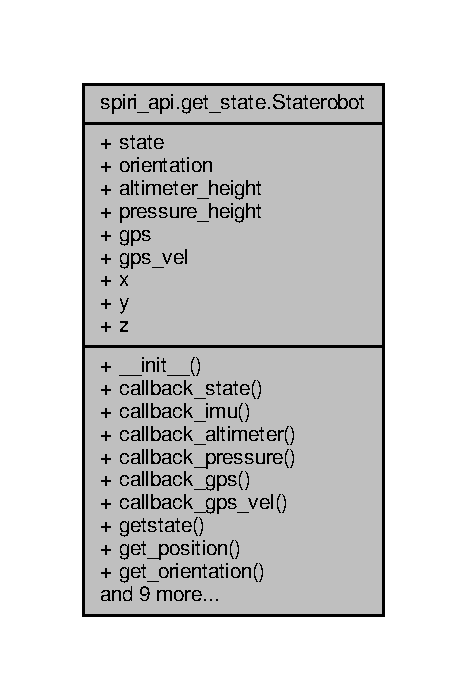
\includegraphics[width=224pt]{classspiri__api_1_1get__state_1_1_staterobot__coll__graph}
\end{center}
\end{figure}
\subsection*{Public Member Functions}
\begin{DoxyCompactItemize}
\item 
def \hyperlink{classspiri__api_1_1get__state_1_1_staterobot_a015efa1f3a59211063e167ec0cb1fc3b}{\-\_\-\-\_\-init\-\_\-\-\_\-}
\begin{DoxyCompactList}\small\item\em Constructor. \end{DoxyCompactList}\item 
def \hyperlink{classspiri__api_1_1get__state_1_1_staterobot_a81570bdf94a8ea111eb9a51b3044c70d}{callback\-\_\-state}
\begin{DoxyCompactList}\small\item\em Callback function for the state topic. \end{DoxyCompactList}\item 
\hypertarget{classspiri__api_1_1get__state_1_1_staterobot_a9136ac9a32b6c7092b3f00ee0fddc3e8}{def \hyperlink{classspiri__api_1_1get__state_1_1_staterobot_a9136ac9a32b6c7092b3f00ee0fddc3e8}{callback\-\_\-imu}}\label{classspiri__api_1_1get__state_1_1_staterobot_a9136ac9a32b6c7092b3f00ee0fddc3e8}

\begin{DoxyCompactList}\small\item\em Callback function for the imu topic. \end{DoxyCompactList}\item 
\hypertarget{classspiri__api_1_1get__state_1_1_staterobot_aee8415185786cc6016fc86bc7e0fcd34}{def \hyperlink{classspiri__api_1_1get__state_1_1_staterobot_aee8415185786cc6016fc86bc7e0fcd34}{callback\-\_\-altimeter}}\label{classspiri__api_1_1get__state_1_1_staterobot_aee8415185786cc6016fc86bc7e0fcd34}

\begin{DoxyCompactList}\small\item\em Callback function for the altimeter topic. \end{DoxyCompactList}\item 
\hypertarget{classspiri__api_1_1get__state_1_1_staterobot_a7597952c4302e24b63fbbc2653221bc9}{def \hyperlink{classspiri__api_1_1get__state_1_1_staterobot_a7597952c4302e24b63fbbc2653221bc9}{callback\-\_\-pressure}}\label{classspiri__api_1_1get__state_1_1_staterobot_a7597952c4302e24b63fbbc2653221bc9}

\begin{DoxyCompactList}\small\item\em Callback function for the pressure\-\_\-height topic. \end{DoxyCompactList}\item 
\hypertarget{classspiri__api_1_1get__state_1_1_staterobot_a42ec392a4f4512781f3a9c0926fdb175}{def \hyperlink{classspiri__api_1_1get__state_1_1_staterobot_a42ec392a4f4512781f3a9c0926fdb175}{callback\-\_\-gps}}\label{classspiri__api_1_1get__state_1_1_staterobot_a42ec392a4f4512781f3a9c0926fdb175}

\begin{DoxyCompactList}\small\item\em Callback function for the fix topic. \end{DoxyCompactList}\item 
\hypertarget{classspiri__api_1_1get__state_1_1_staterobot_a9a9c3e465592be5e619fe5a68a6563a0}{def \hyperlink{classspiri__api_1_1get__state_1_1_staterobot_a9a9c3e465592be5e619fe5a68a6563a0}{callback\-\_\-gps\-\_\-vel}}\label{classspiri__api_1_1get__state_1_1_staterobot_a9a9c3e465592be5e619fe5a68a6563a0}

\begin{DoxyCompactList}\small\item\em Callback function for the fix\-\_\-velocity topic. \end{DoxyCompactList}\item 
\hypertarget{classspiri__api_1_1get__state_1_1_staterobot_af7dfad7d8aed3e97870fb120b8934a59}{def {\bfseries getstate}}\label{classspiri__api_1_1get__state_1_1_staterobot_af7dfad7d8aed3e97870fb120b8934a59}

\item 
def \hyperlink{classspiri__api_1_1get__state_1_1_staterobot_acaa2d63d3153f862a5752ebb75f51a23}{get\-\_\-position}
\begin{DoxyCompactList}\small\item\em A\-P\-I function to read the position x,y,z of Spiri. \end{DoxyCompactList}\item 
def \hyperlink{classspiri__api_1_1get__state_1_1_staterobot_ab8646e99f523f709242d7079a184057e}{get\-\_\-orientation}
\begin{DoxyCompactList}\small\item\em A\-P\-I function to read the orientation of Spiri This function gives the orientation by fusing data from I\-M\-U, G\-P\-S and other sensors. \end{DoxyCompactList}\item 
def \hyperlink{classspiri__api_1_1get__state_1_1_staterobot_a841fe6f1d8d15f7c1aa3022eea33ccdd}{get\-\_\-orientation\-\_\-imu}
\begin{DoxyCompactList}\small\item\em A\-P\-I function to read the orientation of Spiri. \end{DoxyCompactList}\item 
def \hyperlink{classspiri__api_1_1get__state_1_1_staterobot_ac0a65631dbe7edbf353799ca0faab408}{get\-\_\-height\-\_\-altimeter}
\begin{DoxyCompactList}\small\item\em A\-P\-I function to read the altitude of Spiri. \end{DoxyCompactList}\item 
def \hyperlink{classspiri__api_1_1get__state_1_1_staterobot_a9a2667a1295e2b9731614271eb021299}{get\-\_\-height\-\_\-pressure}
\begin{DoxyCompactList}\small\item\em A\-P\-I function to read the altitude of Spiri. \end{DoxyCompactList}\item 
def \hyperlink{classspiri__api_1_1get__state_1_1_staterobot_a1e11c48e95eb0184924776fdbc55b45b}{get\-\_\-gps\-\_\-data}
\begin{DoxyCompactList}\small\item\em A\-P\-I function to read the G\-P\-S data of Spiri. \end{DoxyCompactList}\item 
def \hyperlink{classspiri__api_1_1get__state_1_1_staterobot_af029d50c1f24e86ebfa2aa12d32d9501}{get\-\_\-gps\-\_\-vel}
\begin{DoxyCompactList}\small\item\em A\-P\-I function to read the G\-P\-S velocity of Spiri. \end{DoxyCompactList}\item 
def \hyperlink{classspiri__api_1_1get__state_1_1_staterobot_af6d1fe436714134bbd2fb78da0b09835}{send\-\_\-goal}
\begin{DoxyCompactList}\small\item\em A\-P\-I function to send goals to Spiri. \end{DoxyCompactList}\item 
def \hyperlink{classspiri__api_1_1get__state_1_1_staterobot_abc35e5157bb27bfc35bbfb4aee9df2e5}{send\-\_\-goal\-\_\-relative\-\_\-threading}
\begin{DoxyCompactList}\small\item\em A\-P\-I function to send goals to Spiri. \end{DoxyCompactList}\item 
\hypertarget{classspiri__api_1_1get__state_1_1_staterobot_aa856b1aa2607851f713326fa98aae62f}{def {\bfseries run}}\label{classspiri__api_1_1get__state_1_1_staterobot_aa856b1aa2607851f713326fa98aae62f}

\item 
\hypertarget{classspiri__api_1_1get__state_1_1_staterobot_a26b9c2b42ed90baf83a4b955c5fd8e1c}{def {\bfseries send\-\_\-goal\-\_\-relative}}\label{classspiri__api_1_1get__state_1_1_staterobot_a26b9c2b42ed90baf83a4b955c5fd8e1c}

\end{DoxyCompactItemize}
\subsection*{Public Attributes}
\begin{DoxyCompactItemize}
\item 
\hypertarget{classspiri__api_1_1get__state_1_1_staterobot_ae947739166d346e6aae00131d0ee98a7}{{\bfseries state}}\label{classspiri__api_1_1get__state_1_1_staterobot_ae947739166d346e6aae00131d0ee98a7}

\item 
\hypertarget{classspiri__api_1_1get__state_1_1_staterobot_ad28ef6aa15a4c8b18cf7c70b780800cf}{{\bfseries orientation}}\label{classspiri__api_1_1get__state_1_1_staterobot_ad28ef6aa15a4c8b18cf7c70b780800cf}

\item 
\hypertarget{classspiri__api_1_1get__state_1_1_staterobot_a5af25b2ff39729b5265bb27805dbda10}{{\bfseries altimeter\-\_\-height}}\label{classspiri__api_1_1get__state_1_1_staterobot_a5af25b2ff39729b5265bb27805dbda10}

\item 
\hypertarget{classspiri__api_1_1get__state_1_1_staterobot_a68d6e2d1f4f903fd1661c702cf842c21}{{\bfseries pressure\-\_\-height}}\label{classspiri__api_1_1get__state_1_1_staterobot_a68d6e2d1f4f903fd1661c702cf842c21}

\item 
\hypertarget{classspiri__api_1_1get__state_1_1_staterobot_a47fd76cdbeec362a38d4dfd7249c9eea}{{\bfseries gps}}\label{classspiri__api_1_1get__state_1_1_staterobot_a47fd76cdbeec362a38d4dfd7249c9eea}

\item 
\hypertarget{classspiri__api_1_1get__state_1_1_staterobot_afc80a5b097513a6ddacc889e701639e5}{{\bfseries gps\-\_\-vel}}\label{classspiri__api_1_1get__state_1_1_staterobot_afc80a5b097513a6ddacc889e701639e5}

\item 
\hypertarget{classspiri__api_1_1get__state_1_1_staterobot_af25681493271673605429047bbf12997}{{\bfseries x}}\label{classspiri__api_1_1get__state_1_1_staterobot_af25681493271673605429047bbf12997}

\item 
\hypertarget{classspiri__api_1_1get__state_1_1_staterobot_af85d8f45911429128aae76b7ec00d36a}{{\bfseries y}}\label{classspiri__api_1_1get__state_1_1_staterobot_af85d8f45911429128aae76b7ec00d36a}

\item 
\hypertarget{classspiri__api_1_1get__state_1_1_staterobot_a4365556b013099eef518034e1fd3c0a5}{{\bfseries z}}\label{classspiri__api_1_1get__state_1_1_staterobot_a4365556b013099eef518034e1fd3c0a5}

\end{DoxyCompactItemize}


\subsection{Detailed Description}
Class defining all the functions to control Spiri. 

\subsection{Constructor \& Destructor Documentation}
\hypertarget{classspiri__api_1_1get__state_1_1_staterobot_a015efa1f3a59211063e167ec0cb1fc3b}{\index{spiri\-\_\-api\-::get\-\_\-state\-::\-Staterobot@{spiri\-\_\-api\-::get\-\_\-state\-::\-Staterobot}!\-\_\-\-\_\-init\-\_\-\-\_\-@{\-\_\-\-\_\-init\-\_\-\-\_\-}}
\index{\-\_\-\-\_\-init\-\_\-\-\_\-@{\-\_\-\-\_\-init\-\_\-\-\_\-}!spiri_api::get_state::Staterobot@{spiri\-\_\-api\-::get\-\_\-state\-::\-Staterobot}}
\subsubsection[{\-\_\-\-\_\-init\-\_\-\-\_\-}]{\setlength{\rightskip}{0pt plus 5cm}def spiri\-\_\-api.\-get\-\_\-state.\-Staterobot.\-\_\-\-\_\-init\-\_\-\-\_\- (
\begin{DoxyParamCaption}
\item[{}]{self}
\end{DoxyParamCaption}
)}}\label{classspiri__api_1_1get__state_1_1_staterobot_a015efa1f3a59211063e167ec0cb1fc3b}


Constructor. 

\begin{DoxyRefDesc}{Todo}
\item[\hyperlink{todo__todo000001}{Todo}]The callback needs to be called before the user can send goals.\end{DoxyRefDesc}


\subsection{Member Function Documentation}
\hypertarget{classspiri__api_1_1get__state_1_1_staterobot_a81570bdf94a8ea111eb9a51b3044c70d}{\index{spiri\-\_\-api\-::get\-\_\-state\-::\-Staterobot@{spiri\-\_\-api\-::get\-\_\-state\-::\-Staterobot}!callback\-\_\-state@{callback\-\_\-state}}
\index{callback\-\_\-state@{callback\-\_\-state}!spiri_api::get_state::Staterobot@{spiri\-\_\-api\-::get\-\_\-state\-::\-Staterobot}}
\subsubsection[{callback\-\_\-state}]{\setlength{\rightskip}{0pt plus 5cm}def spiri\-\_\-api.\-get\-\_\-state.\-Staterobot.\-callback\-\_\-state (
\begin{DoxyParamCaption}
\item[{}]{self, }
\item[{}]{data}
\end{DoxyParamCaption}
)}}\label{classspiri__api_1_1get__state_1_1_staterobot_a81570bdf94a8ea111eb9a51b3044c70d}


Callback function for the state topic. 


\begin{DoxyParams}{Parameters}
{\em self} & object pointer \\
\hline
{\em data} & Contains the data published on the topic \\
\hline
\end{DoxyParams}
\hypertarget{classspiri__api_1_1get__state_1_1_staterobot_a1e11c48e95eb0184924776fdbc55b45b}{\index{spiri\-\_\-api\-::get\-\_\-state\-::\-Staterobot@{spiri\-\_\-api\-::get\-\_\-state\-::\-Staterobot}!get\-\_\-gps\-\_\-data@{get\-\_\-gps\-\_\-data}}
\index{get\-\_\-gps\-\_\-data@{get\-\_\-gps\-\_\-data}!spiri_api::get_state::Staterobot@{spiri\-\_\-api\-::get\-\_\-state\-::\-Staterobot}}
\subsubsection[{get\-\_\-gps\-\_\-data}]{\setlength{\rightskip}{0pt plus 5cm}def spiri\-\_\-api.\-get\-\_\-state.\-Staterobot.\-get\-\_\-gps\-\_\-data (
\begin{DoxyParamCaption}
\item[{}]{self}
\end{DoxyParamCaption}
)}}\label{classspiri__api_1_1get__state_1_1_staterobot_a1e11c48e95eb0184924776fdbc55b45b}


A\-P\-I function to read the G\-P\-S data of Spiri. 

This function gives the latitude, longitude, altitude reported by the G\-P\-S Data can be accessed using obj.\-latitude, obj.\-longitude, obj.\-altitude \hypertarget{classspiri__api_1_1get__state_1_1_staterobot_af029d50c1f24e86ebfa2aa12d32d9501}{\index{spiri\-\_\-api\-::get\-\_\-state\-::\-Staterobot@{spiri\-\_\-api\-::get\-\_\-state\-::\-Staterobot}!get\-\_\-gps\-\_\-vel@{get\-\_\-gps\-\_\-vel}}
\index{get\-\_\-gps\-\_\-vel@{get\-\_\-gps\-\_\-vel}!spiri_api::get_state::Staterobot@{spiri\-\_\-api\-::get\-\_\-state\-::\-Staterobot}}
\subsubsection[{get\-\_\-gps\-\_\-vel}]{\setlength{\rightskip}{0pt plus 5cm}def spiri\-\_\-api.\-get\-\_\-state.\-Staterobot.\-get\-\_\-gps\-\_\-vel (
\begin{DoxyParamCaption}
\item[{}]{self}
\end{DoxyParamCaption}
)}}\label{classspiri__api_1_1get__state_1_1_staterobot_af029d50c1f24e86ebfa2aa12d32d9501}


A\-P\-I function to read the G\-P\-S velocity of Spiri. 

This function gives the velocity reported by the G\-P\-S. Data can be accessed using obj.\-x, obj.\-y, obj.\-z \hypertarget{classspiri__api_1_1get__state_1_1_staterobot_ac0a65631dbe7edbf353799ca0faab408}{\index{spiri\-\_\-api\-::get\-\_\-state\-::\-Staterobot@{spiri\-\_\-api\-::get\-\_\-state\-::\-Staterobot}!get\-\_\-height\-\_\-altimeter@{get\-\_\-height\-\_\-altimeter}}
\index{get\-\_\-height\-\_\-altimeter@{get\-\_\-height\-\_\-altimeter}!spiri_api::get_state::Staterobot@{spiri\-\_\-api\-::get\-\_\-state\-::\-Staterobot}}
\subsubsection[{get\-\_\-height\-\_\-altimeter}]{\setlength{\rightskip}{0pt plus 5cm}def spiri\-\_\-api.\-get\-\_\-state.\-Staterobot.\-get\-\_\-height\-\_\-altimeter (
\begin{DoxyParamCaption}
\item[{}]{self}
\end{DoxyParamCaption}
)}}\label{classspiri__api_1_1get__state_1_1_staterobot_ac0a65631dbe7edbf353799ca0faab408}


A\-P\-I function to read the altitude of Spiri. 

This function gives the altitude reported by the Altimeter \hypertarget{classspiri__api_1_1get__state_1_1_staterobot_a9a2667a1295e2b9731614271eb021299}{\index{spiri\-\_\-api\-::get\-\_\-state\-::\-Staterobot@{spiri\-\_\-api\-::get\-\_\-state\-::\-Staterobot}!get\-\_\-height\-\_\-pressure@{get\-\_\-height\-\_\-pressure}}
\index{get\-\_\-height\-\_\-pressure@{get\-\_\-height\-\_\-pressure}!spiri_api::get_state::Staterobot@{spiri\-\_\-api\-::get\-\_\-state\-::\-Staterobot}}
\subsubsection[{get\-\_\-height\-\_\-pressure}]{\setlength{\rightskip}{0pt plus 5cm}def spiri\-\_\-api.\-get\-\_\-state.\-Staterobot.\-get\-\_\-height\-\_\-pressure (
\begin{DoxyParamCaption}
\item[{}]{self}
\end{DoxyParamCaption}
)}}\label{classspiri__api_1_1get__state_1_1_staterobot_a9a2667a1295e2b9731614271eb021299}


A\-P\-I function to read the altitude of Spiri. 

This function gives the altitude reported by the Pressure sensor \hypertarget{classspiri__api_1_1get__state_1_1_staterobot_ab8646e99f523f709242d7079a184057e}{\index{spiri\-\_\-api\-::get\-\_\-state\-::\-Staterobot@{spiri\-\_\-api\-::get\-\_\-state\-::\-Staterobot}!get\-\_\-orientation@{get\-\_\-orientation}}
\index{get\-\_\-orientation@{get\-\_\-orientation}!spiri_api::get_state::Staterobot@{spiri\-\_\-api\-::get\-\_\-state\-::\-Staterobot}}
\subsubsection[{get\-\_\-orientation}]{\setlength{\rightskip}{0pt plus 5cm}def spiri\-\_\-api.\-get\-\_\-state.\-Staterobot.\-get\-\_\-orientation (
\begin{DoxyParamCaption}
\item[{}]{self, }
\item[{}]{format = {\ttfamily 0}}
\end{DoxyParamCaption}
)}}\label{classspiri__api_1_1get__state_1_1_staterobot_ab8646e99f523f709242d7079a184057e}


A\-P\-I function to read the orientation of Spiri This function gives the orientation by fusing data from I\-M\-U, G\-P\-S and other sensors. 

Returns an object. Depending upon the format Euler -\/ Orientation can be accessed using obj.\-x,obj.\-y,obj.\-z Quaternion -\/ obj.\-x,obj.\-y,obj.\-z,obj.\-w 
\begin{DoxyParams}{Parameters}
{\em format} & 1=Quaternion, 0=Euler \\
\hline
\end{DoxyParams}
\hypertarget{classspiri__api_1_1get__state_1_1_staterobot_a841fe6f1d8d15f7c1aa3022eea33ccdd}{\index{spiri\-\_\-api\-::get\-\_\-state\-::\-Staterobot@{spiri\-\_\-api\-::get\-\_\-state\-::\-Staterobot}!get\-\_\-orientation\-\_\-imu@{get\-\_\-orientation\-\_\-imu}}
\index{get\-\_\-orientation\-\_\-imu@{get\-\_\-orientation\-\_\-imu}!spiri_api::get_state::Staterobot@{spiri\-\_\-api\-::get\-\_\-state\-::\-Staterobot}}
\subsubsection[{get\-\_\-orientation\-\_\-imu}]{\setlength{\rightskip}{0pt plus 5cm}def spiri\-\_\-api.\-get\-\_\-state.\-Staterobot.\-get\-\_\-orientation\-\_\-imu (
\begin{DoxyParamCaption}
\item[{}]{self, }
\item[{}]{format = {\ttfamily 'euler'}}
\end{DoxyParamCaption}
)}}\label{classspiri__api_1_1get__state_1_1_staterobot_a841fe6f1d8d15f7c1aa3022eea33ccdd}


A\-P\-I function to read the orientation of Spiri. 

This function gives the orientation reported by the I\-M\-U Depending upon the format Euler -\/ Orientation can be accessed using obj.\-x,obj.\-y,obj.\-z Quaternion -\/ obj.\-x,obj.\-y,obj.\-z,obj.\-w \begin{DoxyReturn}{Returns}
object 
\end{DoxyReturn}

\begin{DoxyParams}{Parameters}
{\em format} & euler=Euler quat=Quaternion \\
\hline
\end{DoxyParams}
\hypertarget{classspiri__api_1_1get__state_1_1_staterobot_acaa2d63d3153f862a5752ebb75f51a23}{\index{spiri\-\_\-api\-::get\-\_\-state\-::\-Staterobot@{spiri\-\_\-api\-::get\-\_\-state\-::\-Staterobot}!get\-\_\-position@{get\-\_\-position}}
\index{get\-\_\-position@{get\-\_\-position}!spiri_api::get_state::Staterobot@{spiri\-\_\-api\-::get\-\_\-state\-::\-Staterobot}}
\subsubsection[{get\-\_\-position}]{\setlength{\rightskip}{0pt plus 5cm}def spiri\-\_\-api.\-get\-\_\-state.\-Staterobot.\-get\-\_\-position (
\begin{DoxyParamCaption}
\item[{}]{self}
\end{DoxyParamCaption}
)}}\label{classspiri__api_1_1get__state_1_1_staterobot_acaa2d63d3153f862a5752ebb75f51a23}


A\-P\-I function to read the position x,y,z of Spiri. 

Returns an object. Position can be accessed using obj.\-x,obj.\-y,obj.\-z \begin{DoxyReturn}{Returns}
Object 
\end{DoxyReturn}
\hypertarget{classspiri__api_1_1get__state_1_1_staterobot_af6d1fe436714134bbd2fb78da0b09835}{\index{spiri\-\_\-api\-::get\-\_\-state\-::\-Staterobot@{spiri\-\_\-api\-::get\-\_\-state\-::\-Staterobot}!send\-\_\-goal@{send\-\_\-goal}}
\index{send\-\_\-goal@{send\-\_\-goal}!spiri_api::get_state::Staterobot@{spiri\-\_\-api\-::get\-\_\-state\-::\-Staterobot}}
\subsubsection[{send\-\_\-goal}]{\setlength{\rightskip}{0pt plus 5cm}def spiri\-\_\-api.\-get\-\_\-state.\-Staterobot.\-send\-\_\-goal (
\begin{DoxyParamCaption}
\item[{}]{self, }
\item[{}]{x, }
\item[{}]{y, }
\item[{}]{z}
\end{DoxyParamCaption}
)}}\label{classspiri__api_1_1get__state_1_1_staterobot_af6d1fe436714134bbd2fb78da0b09835}


A\-P\-I function to send goals to Spiri. 

This function will send a goal with respect to the world. The start position of Spiri is 0,0 \begin{DoxyRefDesc}{Todo}
\item[\hyperlink{todo__todo000002}{Todo}]Return based something on success or failure 

This function should also take in G\-P\-S coordinates 
\begin{DoxyParams}{Parameters}
{\em x} & coordinate in x axis \\
\hline
{\em y} & coordinate in y axis \\
\hline
{\em z} & coordinate in z axis \\
\hline
\end{DoxyParams}
\end{DoxyRefDesc}
\hypertarget{classspiri__api_1_1get__state_1_1_staterobot_abc35e5157bb27bfc35bbfb4aee9df2e5}{\index{spiri\-\_\-api\-::get\-\_\-state\-::\-Staterobot@{spiri\-\_\-api\-::get\-\_\-state\-::\-Staterobot}!send\-\_\-goal\-\_\-relative\-\_\-threading@{send\-\_\-goal\-\_\-relative\-\_\-threading}}
\index{send\-\_\-goal\-\_\-relative\-\_\-threading@{send\-\_\-goal\-\_\-relative\-\_\-threading}!spiri_api::get_state::Staterobot@{spiri\-\_\-api\-::get\-\_\-state\-::\-Staterobot}}
\subsubsection[{send\-\_\-goal\-\_\-relative\-\_\-threading}]{\setlength{\rightskip}{0pt plus 5cm}def spiri\-\_\-api.\-get\-\_\-state.\-Staterobot.\-send\-\_\-goal\-\_\-relative\-\_\-threading (
\begin{DoxyParamCaption}
\item[{}]{self, }
\item[{}]{x, }
\item[{}]{y, }
\item[{}]{z}
\end{DoxyParamCaption}
)}}\label{classspiri__api_1_1get__state_1_1_staterobot_abc35e5157bb27bfc35bbfb4aee9df2e5}


A\-P\-I function to send goals to Spiri. 

This function will send a goal with respect to the start position. Example-\/\-: Suppose Spiri is at 1,1,1 and we call this function send\-\_\-gaol\-\_\-relative(1,0,0). Spiri will move 1 m in x direction. \begin{DoxyRefDesc}{Todo}
\item[\hyperlink{todo__todo000003}{Todo}]Return based something on success or failure 
\begin{DoxyParams}{Parameters}
{\em x} & distance in metres in x axis \\
\hline
{\em y} & distance in metres in y axis \\
\hline
{\em z} & distance in metres in z axis \\
\hline
\end{DoxyParams}
\end{DoxyRefDesc}


The documentation for this class was generated from the following file\-:\begin{DoxyCompactItemize}
\item 
src/spiri\-\_\-api/get\-\_\-state.\-py\end{DoxyCompactItemize}

\hypertarget{classspiri__api_1_1figure__movement_1_1_staterobot}{\section{spiri\-\_\-api.\-figure\-\_\-movement.\-Staterobot Class Reference}
\label{classspiri__api_1_1figure__movement_1_1_staterobot}\index{spiri\-\_\-api.\-figure\-\_\-movement.\-Staterobot@{spiri\-\_\-api.\-figure\-\_\-movement.\-Staterobot}}
}


Collaboration diagram for spiri\-\_\-api.\-figure\-\_\-movement.\-Staterobot\-:
\nopagebreak
\begin{figure}[H]
\begin{center}
\leavevmode
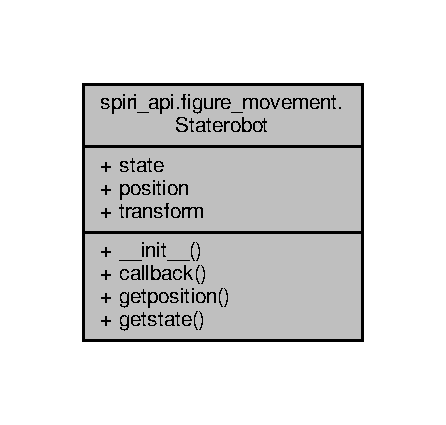
\includegraphics[width=214pt]{classspiri__api_1_1figure__movement_1_1_staterobot__coll__graph}
\end{center}
\end{figure}
\subsection*{Public Member Functions}
\begin{DoxyCompactItemize}
\item 
\hypertarget{classspiri__api_1_1figure__movement_1_1_staterobot_a4bca047e67a87ef60147caa3bec0bfa5}{def {\bfseries \-\_\-\-\_\-init\-\_\-\-\_\-}}\label{classspiri__api_1_1figure__movement_1_1_staterobot_a4bca047e67a87ef60147caa3bec0bfa5}

\item 
\hypertarget{classspiri__api_1_1figure__movement_1_1_staterobot_a321456867de643d09326b856aeec975b}{def {\bfseries callback}}\label{classspiri__api_1_1figure__movement_1_1_staterobot_a321456867de643d09326b856aeec975b}

\item 
\hypertarget{classspiri__api_1_1figure__movement_1_1_staterobot_a745991fc1e78f37812e0065ea177ec53}{def {\bfseries getposition}}\label{classspiri__api_1_1figure__movement_1_1_staterobot_a745991fc1e78f37812e0065ea177ec53}

\item 
\hypertarget{classspiri__api_1_1figure__movement_1_1_staterobot_aa92049eb8526decb28cfa8d34aaa6043}{def {\bfseries getstate}}\label{classspiri__api_1_1figure__movement_1_1_staterobot_aa92049eb8526decb28cfa8d34aaa6043}

\end{DoxyCompactItemize}
\subsection*{Public Attributes}
\begin{DoxyCompactItemize}
\item 
\hypertarget{classspiri__api_1_1figure__movement_1_1_staterobot_a9c09e39041b79d9a85f4e35c2e149b6a}{{\bfseries state}}\label{classspiri__api_1_1figure__movement_1_1_staterobot_a9c09e39041b79d9a85f4e35c2e149b6a}

\item 
\hypertarget{classspiri__api_1_1figure__movement_1_1_staterobot_a4d2c172e525d59802a6fd7379eb149dd}{{\bfseries position}}\label{classspiri__api_1_1figure__movement_1_1_staterobot_a4d2c172e525d59802a6fd7379eb149dd}

\item 
\hypertarget{classspiri__api_1_1figure__movement_1_1_staterobot_a5d011ddfec9b48c254d0e89ede86e8d3}{{\bfseries transform}}\label{classspiri__api_1_1figure__movement_1_1_staterobot_a5d011ddfec9b48c254d0e89ede86e8d3}

\end{DoxyCompactItemize}


The documentation for this class was generated from the following file\-:\begin{DoxyCompactItemize}
\item 
src/spiri\-\_\-api/figure\-\_\-movement.\-py\end{DoxyCompactItemize}

\hypertarget{classspiri__api_1_1request_1_1_staterobot}{\section{spiri\-\_\-api.\-request.\-Staterobot \-Class \-Reference}
\label{classspiri__api_1_1request_1_1_staterobot}\index{spiri\-\_\-api.\-request.\-Staterobot@{spiri\-\_\-api.\-request.\-Staterobot}}
}
\subsection*{\-Public \-Member \-Functions}
\begin{DoxyCompactItemize}
\item 
\hypertarget{classspiri__api_1_1request_1_1_staterobot_ae3e81ac6540cda7ce41cb9ac687cbff6}{def {\bfseries \-\_\-\-\_\-init\-\_\-\-\_\-}}\label{classspiri__api_1_1request_1_1_staterobot_ae3e81ac6540cda7ce41cb9ac687cbff6}

\item 
\hypertarget{classspiri__api_1_1request_1_1_staterobot_a32dd4e20d07c24f5cb292b97088fa1a5}{def {\bfseries callback}}\label{classspiri__api_1_1request_1_1_staterobot_a32dd4e20d07c24f5cb292b97088fa1a5}

\item 
\hypertarget{classspiri__api_1_1request_1_1_staterobot_a7f6d68da682b75115591c6e3889b536e}{def {\bfseries getposition}}\label{classspiri__api_1_1request_1_1_staterobot_a7f6d68da682b75115591c6e3889b536e}

\item 
\hypertarget{classspiri__api_1_1request_1_1_staterobot_ac1be2cdb64902058e65bc90fafead524}{def {\bfseries getstate}}\label{classspiri__api_1_1request_1_1_staterobot_ac1be2cdb64902058e65bc90fafead524}

\end{DoxyCompactItemize}
\subsection*{\-Public \-Attributes}
\begin{DoxyCompactItemize}
\item 
\hypertarget{classspiri__api_1_1request_1_1_staterobot_a273b7ea313a0874c5b9f489cab76e26a}{{\bfseries state}}\label{classspiri__api_1_1request_1_1_staterobot_a273b7ea313a0874c5b9f489cab76e26a}

\item 
\hypertarget{classspiri__api_1_1request_1_1_staterobot_a761f91db29a5269c96a778edfef8985d}{{\bfseries position}}\label{classspiri__api_1_1request_1_1_staterobot_a761f91db29a5269c96a778edfef8985d}

\item 
\hypertarget{classspiri__api_1_1request_1_1_staterobot_aef5196a7d7061152bbb761edcbecad7c}{{\bfseries transform}}\label{classspiri__api_1_1request_1_1_staterobot_aef5196a7d7061152bbb761edcbecad7c}

\end{DoxyCompactItemize}


\-The documentation for this class was generated from the following file\-:\begin{DoxyCompactItemize}
\item 
src/spiri\-\_\-api/request.\-py\end{DoxyCompactItemize}

\printindex
\end{document}
